%%%%%%%%%%%%%%%%%%%%%%%%%%%%%%%%%%%%%%%%%%%%%%%%
% This is the official Latex template prepared for the MSCS program at Weber State Universtiy
% This template is based on the Vanderbilt University Graduate School for submission of dissertations. 
% It is also based on a template originally prepared by Eli Hooten and updated by Haley Adams.

% Using the template is no guarantee that you pass format review with your first submission, but it should save you significant amount of time.

% This template is correct as of September 2021.
%%%%%%%%%%%%%%%%%%%%%%%%%%%%%%%%%%%%%%%%%%%%%%%%

\listfiles
\documentclass[10pt]{report}  %%% Changed from 12pt.

\usepackage[intoc]{nomencl}

\textwidth=6in \oddsidemargin=0.5in \topmargin=-0.5in
\textheight=9in  % 9in must include page numbers
\textfloatsep = 0.4in \addtocontents{toc}{\vspace{0.4in} \hfill
Page\endgraf} \addtocontents{lof}{\vspace{0.2in} \hspace{0.13in} \
Figure\hfill Page\endgraf} \addtocontents{lot}{\vspace{0.2in}
\hspace{0.13in} \ Table\hfill Page\endgraf}

% We've already imported some of the most commonly used packages for inserting formulas, images, tables, and references. If you need more, you can find a list of Latex packages here: https://www.ctan.org/pkg/ 

\usepackage{textcomp}
\usepackage{array}
\usepackage[table, svgnames]{xcolor}
\usepackage{listings}

% -- Defining colors:
\definecolor{codegreen}{rgb}{0.1,0.46,0.1}
\definecolor{codeorange}{rgb}{0.83,0.56,0.26}
\definecolor{codeblack}{rgb}{0.1,0.1,0.1}
\definecolor{codegray}{rgb}{0.95,0.95,0.95}
\definecolor{codepurple}{rgb}{0.58,0,0.82}
\definecolor{backcolour}{rgb}{0.95,0.95,0.92}
\lstdefinestyle{mystyle}{
    backgroundcolor=\color{codegray},   
    commentstyle=\color{codegreen},
    keywordstyle=\color{NavyBlue},
    numberstyle=\tiny\color{codeblack},
    stringstyle=\color{codeorange},
    basicstyle=\ttfamily\footnotesize\bfseries,
    breakatwhitespace=false,         
    breaklines=true,                 
    captionpos=t,                    
    keepspaces=true,                 
    numbers=left,                    
    numbersep=5pt,                  
    showspaces=false,                
    showstringspaces=false,
    showtabs=false,                  
    tabsize=2
}
\lstset{
  style=mystyle,
  framexleftmargin=3.5mm,
  frame=box,
  rulesepcolor=\color{black},
  linewidth=\linewidth,
  xleftmargin=12pt,
  aboveskip=12pt,
  belowskip=12pt
}

\usepackage{setspace}
\usepackage{mathptmx}
\usepackage{colortbl}
\usepackage{graphicx}
\usepackage{amssymb, amsmath}
\usepackage{subfig}
\usepackage{epsfig}
\usepackage{times}
\usepackage{float}
\usepackage{rotating}
\usepackage{makeidx}
\usepackage{url}
\usepackage{multirow}
\usepackage{booktabs}
\usepackage{tabularx}
\usepackage{xspace}

\usepackage[subfigure, titles]{tocloft}
\usepackage{acronym}
\usepackage{datetime}


%%another algorithm package
\usepackage{algorithm}
\usepackage{algorithmic}

\renewcommand{\nomname}{LIST OF ABBREVIATIONS}
\makenomenclature

\graphicspath{{Figures/}}
\DeclareGraphicsExtensions{.pdf,.jpeg,.png,.PNG, .eps, .tiff}


\usepackage{makecell}
\usepackage{titletoc}
\usepackage{sfchap}
\usepackage{sfsection}
\usepackage{cite}
\usepackage[numbers]{natbib}
%\usepackage[nottoc]{tocbibind}
%\usepackage[authoryear]{natbib}
%\usepackage{apacite}
\usepackage{appendix}
%\usepackage{tocbibind}

%
\setcounter{secnumdepth}{7}
\setcounter{tocdepth}{7}

\usepackage[hidelinks,colorlinks=true,linkcolor=blue,citecolor=blue]{hyperref}
\hypersetup{
    colorlinks=true,
    linkcolor=blue,
    filecolor=magenta,      
    urlcolor=cyan,
    pdftitle={Building Resource Adaptations via Test-Based Software Minimization},
    pdfpagemode=FullScreen,
}%
\urlstyle{same}

\usepackage[all]{hypcap}

% Stats table label
\newcommand{\statslabel}[2]{\multirowcell{#1}[-1.6mm][c]{#2}}

% Below heading rule.
\newcommand{\otoprule}{\midrule[\heavyrulewidth]}

% Prevent double spaced equations
\newenvironment{tightequation}{\singlespace\begin{equation}}{\end{equation}}

% Project Name
\newcommand {\mytool}{ReduSharptor\xspace}

% Extra junk to pretty up the table of contents
\setlength{\cftsecnumwidth}{2.8em}
\setlength{\cftsubsecnumwidth}{3.7em}
\setlength{\cftsubsubsecnumwidth}{4.6em}
\setlength{\cftparanumwidth}{5.5em}
\setlength{\cftsubparanumwidth}{6.5em}
\setlength{\cfttabnumwidth}{3.5em}
\setlength{\cftfignumwidth}{3.5em} 

\renewcommand{\contentsname}{TABLE OF CONTENTS}
\renewcommand{\listfigurename}{LIST OF FIGURES}
\renewcommand{\listtablename}{LIST OF TABLES}
\renewcommand{\bibname}{ \texorpdfstring{{References\vspace{10mm}}}{References}   }
%
\renewcommand{\chaptermark}[1]{%
  \markboth{\MakeUppercase{%
      \chaptername}\ \thechapter.%
    \ #1}{}}
    
    
\interfootnotelinepenalty=10000 %prevents the splitting of long footnotes across multiple pages. Use with caution. 

\begin{document}

%%%%%%%%%%%%%%%%%%%%%%%%%%%%%%%%%%%%%%%%%%%%%%%%%%%%%%%%%%%%%%%%%%%%%%%%%%%%%%%%
%% Prevent the warning: pdfTeX warning (ext4): destination with the same identifier (name{page.1}) has been already used, duplicate ignored
%%	This setting will make a difference to the output because the page number is suppressed for the title page
\pagenumbering{alph}



 
\begin{titlepage}
\thispagestyle{empty}\enlargethispage{\the\footskip}%
\begin{center}
    \hspace{1em}\vspace{6em} \\ % add space before content
	{\setstretch{1.66} \MakeUppercase{Simplification of developer-written C\# unit tests}\par }
	\vskip.2in
	By
	\vskip .2in
	{David Weber}
	\vskip .2in
	
	\begin{doublespace}
	A thesis\\  
		Submitted to the faculty of the \\ 
		MSCS Graduate Program of Weber State University\\
		in partial fulfillment of the requirements \\
		for the degree of \\ [.2in]
	\end{doublespace}
	
	MASTER OF SCIENCE \\[.1in]
	in \\[.1in]
	Computer Science \\[.1in]
	December 16, 2022 \\[.2in]
	%%%The date will reflect your proposed degree conferral date as selected from the Intent to Graduate form. This is your actual graduation date, not your thesis or defense date.%%%
	
	Ogden, Utah
	\vskip .5in
\end{center}


%%%Uncomment for Signatures%%%
\begin{doublespace}
Approved: \hskip 2.5in Date:\\[1.2em]
\rule{3.5in}{.5pt} \hskip 0.1in \rule{2in}{.5pt} \\[.1in]
Committee Chair, Arpit Christi, Ph.D. \\  [.2in]
\rule{3.5in}{.5pt} \hskip 0.1in \rule{2in}{.5pt} \\[.1in]
Committee member, Yong Zhang, Ph.D. \\ [.2in]
\rule{3.5in}{.5pt} \hskip 0.1in \rule{2in}{.5pt} \\[.1in]
Committee member, Nicole Anderson, PhD. \\ [.2in]
%\rule{3.5in}{.5pt} \hskip 0.1in \rule{2in}{.5pt} %\\[.1in]
\end{doublespace}
%%%%%%%%%%%%%%

%%%%%%Uncomment  for Approved Names%%%%%%
%\begin{center}
%\begin{doublespace}
%Approved:\\ [.2in]
%Committee Chair, Ph.D. \\  [.2in]
%Committee member, Ph.D. \\ [.2in]
%Committee member, Ph.D. \\ [.2in]
%Committee member, Ph.D.
%\end{doublespace}
%\end{center}

\end{titlepage}


%%%%%%%%%%%%%%%%%%%%%%%%%%%%%%%%%%%%%%%%%%%%%%%%%%%%%%%%%%%%%%%%%%%%%%%%%%%%%%%%
\doublespacing
\pagenumbering{roman} \setcounter{page}{2}

% These 3 sections are optional 
\singlespacing  
%\doublespacing % Single or Double spacing for these sections?

%%%%%%%%%%%%%%%%%%%%%%%%%%%%%%%%%%%%%%%%%%%%%%%%%%%%%%%%%%%%%%%%%%%%%%%%%%%%
\chapter*{ACKNOWLEDGMENTS}
\addcontentsline{toc}{chapter}{ACKNOWLEDGMENTS}
\vspace{7mm}

I would like to thank my committee chair, Dr. Arpit Christi, and my committee members, Dr. Yong Zhang, and Dr. Nicole Anderson, for their guidance and support throughout the course of this research.
In addition, I would also like to thank Chelsea Johnson, Nathan Cummings, and additional friends and family for their support during the course of this research.
. 


%%%%%%%%%%%%%%%%%%%%%%%%%%%%%%%%%%%%%%%%%%%%%%%%%%%%%%%%%%%%%%%%%%%%%%%%%%%%
\chapter*{ABSTRACT}
\addcontentsline{toc}{chapter}{ABSTRACT}
\vspace{7mm}

Modern software systems are complex and locating, isolating and fixing a fault even with a failing test is tedious and time-consuming. Simplifying failing test(s) can significantly reduce the developer effort by reducing the irrelevant program entities that developers need to observe. Delta Debugging (DD) algorithms automatically reduce the failing tests. Hierarchical Delta Debugging (HDD) algorithms improve DD for hierarchical tests like source code and HTML files. Many modern implementations of these algorithms work on a generic tree-like structure and fail to consider complex structures, intricacies, and interdependence of program elements of a particular programming
language. We propose a tool, \mytool, to simplify C\# tests that uses language-specific features and interdependence of C\# program elements using Roslyn compiler APIs. We evaluate the tool on a set of 30 failing C\# tests to demonstrate its applicability and accuracy.     

 


%%%%%%%%%%%%%%%%%%%%%%%%%%%%%%%%%%%%%%%%%%%%%%%%%%%%%%%%%%%%%%%%%%%%%%%%%%%%%%%%
\singlespacing
\tableofcontents

%%%%%%%%%%%%%%%%%%%%%%%%%%%%%%%%%%%%%%%%%%%%%%%%%%%%%%%%%%%%%%%%%%%%%%%%%%%%%%%%
\begingroup
\setlength{\parskip}{1\baselineskip}
\listoftables
\newpage
\listoffigures
\newpage
%\printnomenclature %list of abbreviations is optional
%\newpage
\endgroup

%%%%%%%%%%%%%%%%%%%%%%%%%%%%%%%%%%%%%%%%%%%%%%%%%%%%%%%%%%%%%%%%%%%%%%%%%%%%%%%%
\normalsize
\doublespacing

%%%%%%%%%%%%%%%%%%%%%%%%%%%%%%%%%%%%%%%%%%%%%%%%%%%%%%%%%%%%%%%%%%%%%%%%%%%%
\chapter*{Contribution of Authors}
\addcontentsline{toc}{chapter}{Contribution of Authors}
\vspace{7mm}

The following authors contributed to the manuscript: David Weber (DW), Arpit Christi (AC)

\begin{table}[h]
\caption{Author Contributions}
\begin{center}
{\scriptsize
\begin{tabular}{|l|l|l|l|l|}
\hline
Task & Conception & Data Collection & Empirical Analysis & Final Draft \\
\hline
\hline
{Thesis} & {DW, AC} & {DW} & {DW} & {DW, AC} \\
\hline

\end{tabular}
}
\end{center}
\label{contributionOfAuthors}
\end{table}

This study is currently under consideration in the SANER 2023 tools track conference. This conference is a CORE-A conference~\cite{core_conference_portal} and will allow for additional opportunities for \mytool to show its usefulness.


 

\pagenumbering{arabic}
\setcounter{page}{1}



\chapter{Introduction} \label{CH1_Introduction}
%\vspace{-7mm}
%\bigskip

The complexity of modern software makes debugging difficult and time consuming. To debug a failing program, the developer needs to locate and isolate the fault first; a slow and tedious process known as Fault Localization (FL). If the failing tests only execute a few faulty program elements, FL is trivial. The complexity arises from the fact that failing tests often execute a large set of non-faulty program elements. Hence, simplification of failing tests, while keeping the bug, reduces the complexity of fault localization by reducing the number of non-faulty program elements the developers need to search. It focuses developers' attention on a few faulty program elements, leading to faster debugging times. Simplified failing tests are not only helpful aid to developers, it can significantly improve the accuracy of automatic fault localization techniques~\cite{vince2021reduction,christi18reduce}. These automatic fault localization techniques have the goal of automatically finding the faulty program elements without the need of a developer to search through them. While a long, complex, failing test leads to longer execution times for these techniques, simplifying the unit tests before this step reduces the execution time significantly.

The most widely known and utilized automatic test simplification technique is the Delta Debugging (DD) algorithm, by Zeller and HildeBrandt. This algorithm works well on test inputs that can be considered array or list-like structures~\cite{zeller2002simplifying}. Additionally, it is not the most effective technique for tests that have tree-like structures as seen in HTML files, C or java programs, or XML files. This is due to the fact that it only works on a flat structure, or in other words, will not break apart smaller blocks in order to simplify those sections as well. However, Mishreghi and Su proposed the Hierarchical Delta Debugging (HDD) algorithm that utilizes the underlying Abstract Syntax Tree (AST) structure to effectively simplify these unit tests. ~\cite{misherghi2006hdd}. 

Recently, a few researchers proposed modern implementations of HDD algorithms and their variants~\cite{hodovan2016modernizing, perses, gopinath2020abstracting, stepanov2019reduktor}. Most of the implementations are language-agnostic and, hence, can reduce a variety of tests in languages such as HTML, XML, C, or java. Stepanov et al. noted the language-agnosticism of the HDD tools. This is a major limiting factor in employing the tools efficiently for real-world, large-scale usage as the tools fail to consider and utilize the language-specific features, complexities, and inter-dependencies~\cite{stepanov2019reduktor}. These tools rely on a generic AST or grammar in the simplification process and produce many noncompilable intermediate variants before the convergence. Sun et al. noted the need of producing syntactically correct intermediate test variants while proposing the \emph{Perses} algorithm~\cite{perses}. Also, most of the tools rely on many libraries, components, and external tools that need to be up-to-date all the time to utilize the tools. Binkley et al. argue that the cost of development and maintenance is prohibitive for program slicing tools (DD/HDD produces a slice) due to the need of a large set of libraries and components~\cite{binkley2014orbs}. Many of these tools require a certain preprocessing step before they can be utilized to simplify tests~\cite{perses, hodovan2016modernizing}. 

Instead of focusing on varying sets of test inputs and test cases, the focus was on \emph{developer-written} \emph{C\#} unit tests. As we focused our attention, observed, and studied unit tests implemented in C\# by developers, we noticed that we can utilize new avenues to implement a test reduction tool that is applicable, accurate, and easy to use. 

To this end, we propose a tool, \mytool, that provides the following: 

\begin{enumerate}
    \item A tool specifically implemented for C\# tests that utilizes language-specific features of C\# programs and tests. 
    \item A tool that utilizes an empirical analysis to prune the search space.
    \item A tool that exists as a stand-alone entity and does not require any further libraries or tool sets. This tool can be invoked using an executable file. 
    \item A tool that requires absolutely no preprocessing steps.
\end{enumerate}

We evaluate \mytool on a set of 30 failing tests on 5 open source C\# projects to demonstrate that \mytool is applicable and accurate. The tool can produce correct test simplifications with high precision (96.58\%) and recall (96.45\%). \mytool is publicly available on GitHub.











\clearpage % clear the prior chapter's page

\chapter{Related Work}\label{CH2_RelatedWork}
%\vspace{-7mm}
%\bigskip

\section{DD and HDD}
There are several different algorithms used to simplify unit tests or code bases. One of which is DD, an algorithm that simplifies failing tests while still keeping the bug. This algorithm works by utilizing a variant of binary search to remove individual components that are unnecessary for triggering the bug~\cite{zeller2002simplifying}. To retrofit DD for hierarchical test inputs like XML, HTML, or programs, the top syntax tree is used as a flat structure. This means the elements would include blocks of nested elements for removal. This method is faster and more efficient than other algorithms since it doesn't entail further nested elements but means that it is much more limited since it cannot find further unneeded statements within deeper code blocks. It cannot find these statements because the algorithm treats these code blocks as a single statement, meaning it removes the entirety of the block or none at all. This is relevant since many algorithms that need to be reduced have tree-like structures, meaning this algorithm cannot effectively simplify every test.

The DD algorithm works by separating a portion of code into smaller sections. By testing these sections in certain ways, we are able to find statements that do not need to be kept for the failing logic to remain. If we remove these statements and continue the process until no more statements can be removed, we will end up with the simplified failing test. We start with a certain number of sections and test each individually. If any of these tests fail, we use that as the new input. If all of these sections' tests succeed or cannot compile, we continue searching. After testing each of these, we will test the compliment of each section, or the combination of every other section. Likewise, if we find a failing configuration, we use that as the new input. If all of these configurations fail, we increase the granularity until the number of sections exceeds the number of statements remaining.

While DD is useful alone, it is not effective for all situations. One situation was further investigated by Misherghi and Su, who proposed that HDD works effectively on tree-like inputs by exploiting the underlying AST~\cite{misherghi2006hdd}. This AST allows for the HDD algorithm to break down the blocks of code into smaller blocks of code, thus allowing for the algorithm to run recursively and find additional unneeded statements for removal. The primary concern with using this approach comes from the increased time, and therefore more resources, needed to parse these AST structures. While both DD and HDD are theoretically sound algorithms that guarantee convergence and minimalism, HDD is able to break down the statements further, allowing for more effective simplification. 

The HDD algorithm is useful for finding and reducing code and tests within a tree structure. This algorithm works by breaking down the statements recursively by blocks of code. It then runs the DD algorithm at every level in a postorder traversal, or in other words, it starts with the inner-most layer. If a block needs to be removed entirely, it will do so while simplifying a layer above it. Take a look at figure~\ref{fig:hddFigure} for pseudo-code behind the HDD algorithm.

\begin{center}
\begin{figure}[!ht]
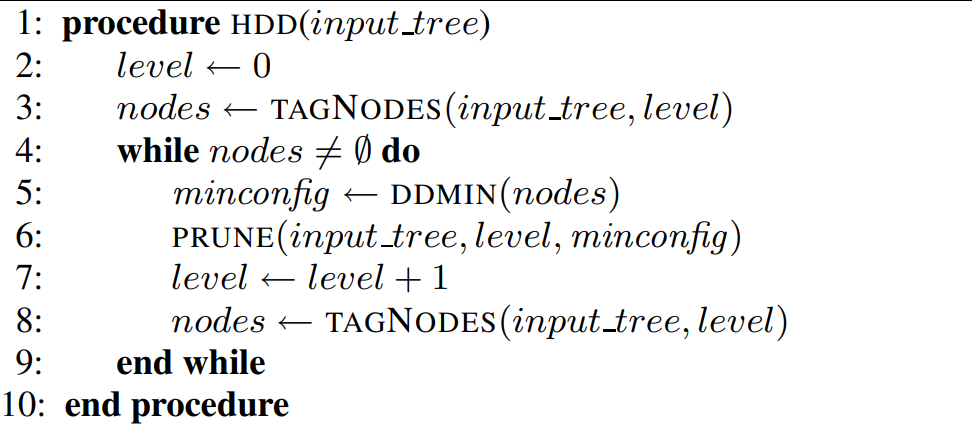
\includegraphics[width=\linewidth]{hddFigure.png}
\caption{HDD algorithm~\cite{misherghi2006hdd}}
\label{fig:hddFigure}
\end{figure}
\end{center}

Regehr et al. proposed C-Reduce to simplify tests for C compiler testing that uses DD as a starting point and further generalizes it. They also look into the test case validity problem to handle undefined and unspecified behavior. Their work showed significant improvement in simplifying C compiler tests that were produced by C-Smith (a random testing tool for C compiler testing) compared to other approaches~\cite{regehr2012test}.

Fuzzers are random testing mechanisms. When fuzzers are used to find bugs, they tend to find the same bugs repetitively. This makes it harder to find diverse bugs early. Fuzzer taming is used to make fuzzers produce more diverse bugs early or to categorize the bugs such that different bugs fall into different categories. Pei et al. combined delta-debugging trails with Furthest Point First algorithm to produce diverse bugs early~\cite{7022682}.

While simplifying tests with DD algorithms can help find underlying bugs in code bases, it still needs existing tests to be able to catch these bugs. Alex Groce et al. avoids this limitation with \emph{cause reduction}~\cite{groce_alipour_zhang_chen_regehr}. \emph{Cause reduction} utilizes the DD algorithm to simplify test cases with respect to arbitrary effects in order to provide quick tests for real-world programs. In other words, \emph{cause reduction} can help find bugs by exploring additional branches of variants that normally would not be explored by the regular DD algorithms. These additional variants provide more areas for potential bugs without a need for a unit test. Therefore, this has the potential to be more effective at finding bugs than previous approaches. 

\section{Additional resources}
Even though HDD was able to create a tree structure, it did not do anything about changing the structure of the syntax tree. This would lead the tree to be imbalanced at times, making a situation not ideal for the HDD algorithm. Using this algorithm with an unbalanced tree is inefficient and resource intensive. This led Hodovan and Kiss to research further, and claim that Extended Context Free Grammar with HDD produces a more balanced tree than one produced by a Context Free Grammar. In other words, by changing the way these statements are parsed, it can create a more balanced tree, leading to a more efficient situation. They then utilized it in implementing a modernized HDD tool called picireny~\cite{hodovan2016modernizing}. 

While the DD and HDD algorithms are effective with simplification, there is potential for better algorithms. In order to have both effectiveness and efficiency, you need to implement both algorithms, and this will still only provide one benefit or the other. In an effort to address this issue, Herfert et al. proposed an additional algorithm known as the Generalized Tree Reduction (GTR) algorithm. The GTR algorithm relies on operations other than removal or deletion and replacing a tree node with a similar tree node~\cite{Herfert2017GTR}. This presented an effective alternative to DD and presented the idea that DD/HDD is not the only syntax tree simplification option. This different approach to the problem is a great demonstration that there are still many potential improvements that have not been discovered yet. 

While all these resources find ways of providing alternatives or different approaches to the HDD algorithm, there are still plenty of other areas for performance boosts. These algorithms are slow and resource intensive, and in need of performance enhancements. Sun et al. noticed this issue which led them to research further. They observed that during the simplification process, many previous algorithms produced \emph{syntactically invalid variants}. These \emph{syntactically invalid variants} are variations of the code that will not even pass a simple compilation step. However, a futile compilation step still needs to be performed before pruning the invalid variant. They proposed the \emph{Perses} algorithm specifically to avoid generation of these invalid variants~\cite{perses}. By knowing about these \emph{syntactically invalid variants} before compiling, it makes the application of these algorithms more time efficient since it reduces the amount of time compiling each variant.

While the DD and HDD algorithms provide a solution for test simplification, there are still other enhancements that can be made. Gopinath et al. utilized the \emph{Perses} algorithm to propose the \emph{DDSET} algorithm to abstract minimal failure-inducing input from a larger set using input grammar~\cite{gopinath2020abstracting} creating an additional simplification algorithm. This new algorithm is very efficient and reduces time needed to simplify. This is a very unique approach to the problem and gives another alternative for unit test simplification through generalization of the algorithm and only allowing \emph{syntactically valid} variants.

A large problem with the research so far is the level of abstraction with it. There are several different languages that each provide their own syntax, creating issues with each specific language. This led \emph{Picireny}, \emph{Perses}, and \emph{DDSET} to use Antlr, a powerful parser generator, to produce the AST for specific programming languages~\cite{parr}. Antlr provides the ability to produce a parser for several programming languages without creating each individually. This is a significant tool to use for problems regarding programming languages in general since this will provide a parser for each, giving the option to implement these solutions in a variety of languages.

Binkley et al. proposed another useful resource as the \emph{Observational-based Slicing} (ORBS) technique. This technique uses program line deletion as a fundamental operation to slice programs accurately and efficiently~\cite{binkley2014orbs}. This deletes potential slices of the program and observes and compares the behavior of the program before and after deletion. If the program behaves the same in both the original and the slice, then the deletion is kept. While this concept is not very complex, it provides an additional solution to these simplification problems and opens the door for more ideas to be implement.

An additional resource came from Christi et al. when they combined inverted HDD with statement deletion mutation to simplify programs for the purpose of resource adaptations. They argued that reduction is only meaningful and useful at statement level and avoided non-statement level reductions~\cite{christi2017saso, christi2018qrs}. By only focusing on statements specifically instead of lines generated, there are a significant number of skipped variants that will not compile. Non-statement level reductions can lead to partial statements that cannot compile. By focusing on entire statements, we are able to skip these partial statements and increase efficiency. This approach will still reduce and simplify the same, but provides an alternative to not spend time on compilation for these variants. By doing this, they presented the perspective that simplification performance can be efficient by simply focusing on statement reduction.


\clearpage % clear the prior chapter's page

\chapter{Motivation}\label{CH3_Motivation}
%\vspace{-7mm}
%\bigskip


\begin{figure}
\begin{lstlisting}[language=C, linewidth=0.6\linewidth]
[Fact]
public void ApplySomeArgs()
{
	var opt = Some(add)  // 1
		.Apply(Some(3))   // 2
		.Apply(Some(4));  // 3

	Assert.Equal(Some(7), opt);  // 4
}
\end{lstlisting}

\caption{\texttt{ApplySomeArgs} test in \texttt{language-ext}}
\label{fig:applySomeArgs}
%\vspace{-0.5in}
\end{figure}


\section{Purpose of the minimized test}
If test minimization is used for compiler testing, even a noncompilable piece of source code can be a useful artifact in debugging and bug isolation. Our focus is to reduce the failing unit tests to aid developers in debugging. Hence, the end product of test simplification must be compilable and executable tests that remain with the same failing logic. Any intermediate test that has compilation errors will be pruned and will not be used for further processing by the simplification process since the tool cannot produce a pass/fail result on such a test.


\section{The cost of compilation}
Whenever any changes are made in either the program or test, the source code needs to be compiled before executing the test. In test reduction, we always modify or reduce the test. Hence, the test project, library, or jar needs recompilation. For real-world test projects, the compilation time can be very high. For example, after a change is made in any of the tests, the \texttt{language-ext} project has a compilation time of approximately 11 seconds on a Windows machine with Intel(R) Core(TM) i7-8650U CPU @ 1.90GHz processor and 16.0 GB RAM. 


\section{Performance of other techniques}
Since there are other techniques used for simplification, there are possibilities of better performance using one of those. However, if we simulate the behavior of the \emph{ORBS} or \emph{Perses} techniques on the provided test~\cite{fig:applySomeArgs}, we notice the potential of producing more variants that cannot compile. Therefore, while there are still noncompilable variants within this example, there is no alternative that provides a better approach.

The \emph{ORBS} technique relies on line-level reduction and, hence, it may produce variants where line 1 or line 3 are removed from the test; both of which are noncompilable. The \emph{Perses} technique attempts to produce a syntactically correct variant, but syntactic correctness does not always result in successful compilation. For example, in line 2, \texttt{.Apply(Some())} and \texttt{.Apply()} are syntactically correct variants, but are still noncompilable. The \emph{Perses} technique will produce many such variants for the given test leading to more time put into compilation.


\section{Using statements as the unit of reduction}
Instead of using nodes in the AST or lines in the test file as the basis of reduction, \mytool uses program statements for the unit of reduction. The statement is defined by the \texttt{StatementSyntax} class or other derived classes of the Roslyn compiler API class~\cite{wagner_2021}. With statements as the unit of reduction, lines 2, 3, and 4 will be treated as a single statement of type \texttt{LocalDeclarationStatementSyntax} by the Roslyn compiler. Hence, It can only produce one variant that cannot compile - the variant where the entire first statement is deleted. This results in fewer noncompilable variants to be tested, meaning less time wasted on compilation in general.

\section{Fewer intermediate variants}
When we use statements as the unit of reduction, we are essentially considering the AST with significantly less nodes because we ignore the existence of nodes below the statement level. As the DD/HDD algorithm will have to process fewer nodes, a large number of variants will be pruned automatically, resulting in considerable reduction in the search space. Therefore, less time will be required to simplify the test because a large number of variants will not need to be compiled and tested.

\section{DD is sufficient}
Consider the fictitious test case shown in figure~\ref{fig:foo}. The corresponding AST representation is available in figure~\ref{fig:ast}. The figure only shows statement nodes as we already argued for not using nodes below the statement level. Now consider two nodes that correspond to lines 1 and 2 of figure~\ref{fig:foo}. Such statements do not have a sub tree with our statement deletion assumptions. The \texttt{if} statement spanned across lines 3, 4, and 5 results in a tree. We divide the Roslyn compiler statement sets into two distinct sets: \emph{NonTree} statements that \emph{cannot} form sub trees, and \emph{Tree} statements that \emph{can} form sub trees. We conducted an empirical analysis on 1000 distinct developer written unit tests and observed the statement usage. We found \emph{Tree} statements are infrequent in \emph{developer-written} C\# unit tests. Therefore, we will consider a \emph{Tree} statement to be a \emph{NonTree} statement. We will process the \texttt{if} statement as a single statement instead of processing the corresponding sub tree. For the figure~\ref{fig:foo} code, this means treating lines 3, 4, and 5 as a single statement. Either the entire block is removed or nothing is removed. We don't have any chance to separately process the \texttt{Assert} statement in line 4. This approach provides two advantages: fewer statements need to be processed, and all statements below block statements are considered \emph{Tree} statements. We have a list or set of  \emph{NonTree} statements below the block statement level, and we can process them using the DD algorithm with $O(n^2)$ complexity instead of the HDD algorithm with $O(n^3)$ complexity. At first glance, we seem to be sacrificing accuracy for efficiency in the entire process, however, our results demonstrate that such simplification works well in practice. 

\clearpage % clear the prior chapter's page

\chapter{\mytool: Usage, Architecture, and Implementation Details}\label{CH4_ToolUsage}
%\vspace{-7mm}
%\bigskip

\section{Usage}
For ease of this experiment, we have created a tool, \mytool~\cite{weber_2022}, that will simplify the unit tests. To use this tool, the developer will only have to provide the following: test file with full path, name of the test (as a single file can have many tests and we may want to reduce only one failing test), and the path of the \texttt{.csproj} file associated with the code. All of this information is already available to the developers. Optionally, the developer can provide a particular folder path if they want to use it to store intermediate results and the final output in that folder. An example of this execution can be seen in figure~\ref{fig:command}. The architecture from a developer's perspective is described in figure~\ref{fig:tool_architecture}. If you compare the architecture figure with the \emph{Perses} workflow figure and the \emph{Picireny} architecture figure, the contrast is clear~\cite{hodovan2016modernizing, perses}. Both the \emph{Perses} and \emph{Picireny} approaches require significant preprocessing steps that require other libraries, toolsets, and components. Both of them require a test script to be available, normally a shell file or a batch file. \mytool does not require any of these as explained in the architecture section. 

\begin{figure*}
\begin{lstlisting}
ReduSharptor.exe ".\language-ext\LanguageExt.Tests\ApplicativeTests.cs" "ListCombineTest" ".\language-ext\LanguageExt.Tests\LanguageExt.Tests.csproj" ".\Simplified Test Results"
\end{lstlisting}
\caption{\texttt command line execution of \mytool}
\label{fig:command}
%\vspace{-0.5in}
\end{figure*}

\begin{center}
\begin{figure}[!ht]
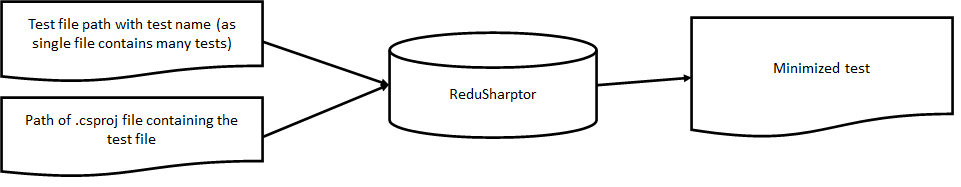
\includegraphics[width=\linewidth]{tool_archicture.png}
\caption{\mytool architecture from a user's perspective}
\label{fig:tool_architecture}
\end{figure}
\end{center}

\section{Architecture}
As \mytool is implemented for C\#, it takes into consideration how C\# programs are organized using \texttt{.sln} and \texttt{.csproj} files. In order to compile or run the test, \mytool uses the \texttt{.csproj} file, the test, and the built-in build+run utility available as part of the \texttt{.NET} framework and Roslyn compiler to generate the necessary build+run script. The process is described in the right side of figure~\ref{fig:internal}. On the left side, we describe how a test is processed first using the Roslyn compiler to generate the parse tree. The parse tree will go through a pruning and transformation process to produce a tree where \emph{Tree} statements will be processed as \emph{NonTree} statements. The test, the processing statement list, and the build+run script will then be passed to the DD algorithm to produce the minimized test. The \emph{Perses} and \emph{Picireny} approaches require the user of their tool to provide a test script which may increase in complexity over time as both approaches will require a new test script for each test minimization. 

\begin{center}
\begin{figure}[!ht]
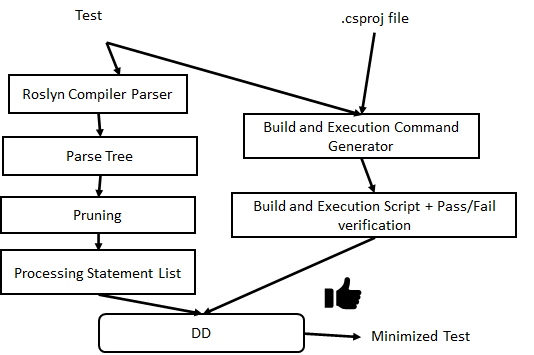
\includegraphics[width=\linewidth]{internal_architecture.png}
\caption{\mytool internal architecture with implementation details}
\label{fig:internal}
\end{figure}
\end{center}

In addition, a great effort was made to not have any external dependencies, libraries, or tool sets and, as a result, \mytool only utilizes the \texttt{.NET} framework and Roslyn compiler API, which is available as part of the \texttt{Microsoft.CodeAnalysis} library. Therefore, a user can easily invoke \mytool as a command line utility without the needing to download or maintain any external components or libraries. Because \mytool is a C\# specific tool designed for C\# unit tests, the need for preprocessing steps is eliminated.

\section{Implementation}

The execution of the simplification process is rather simple. It separates the tests into sections of statements and attempts to run each section as a standalone test. If any of the sections result in a failed test, that section is made the new test and the process is repeated. Otherwise, the complement of each section is attempted and, likewise, is made the new test if any of them fail. If none of the sections or their complements fail, then the granularity of the sections is increased and the process is repeated. This process is continued until all sections result in successful runs and the sections cannot be reduced any further. This is an adapted form of the work of A. Zeller et al.~\cite{zeller2002simplifying}. However, instead of using a set of failing input values, this approach simplifies and isolates the unit test statements themselves.

In \mytool, this primary simplification code exists within the \texttt{FindSmallestFailingInput} method from figure~\ref{fig:FindSmallestFailingInput1}. Each \texttt{foreach} block tests the sections and their complements and are then checked to see if any of the tests are successful. Following those blocks, the granularity of the sections is increased on line 51, then checked against the number of remaining statements to ensure the number of sections does not exceed the amount of statements. If the level of granularity if more than the remaining statements, then the simplification process is finished.

In order to understand the tool fully, a great understanding must be had about how these algorithms were originally implemented. In figure~\ref{fig:Main1} rests the \mytool entry point, the \texttt{Main} method. After taking input from the command line arguments, this gets the statements from the provided unit test and creates a copy as a backup. The \texttt{Main} method then calls \texttt{FindSmallestFailingInput}, which starts the simplification algorithm. After producing the simplified output, it reverts the test file to its original state and outputs the simplified statements into a separate file.

The Roslyn compiler is used in a few of the methods: figures~\ref{fig:GetTestStatements1}, \ref{fig:SetTestStatements1}, and \ref{fig:GetTestCallString1}. \texttt{GetTestStatements} and \texttt{SetTestStatements} both use Roslyn in similar ways to break apart the file and find the unit test from a name, however, \texttt{SetTestStatements} also uses Roslyn in order to write a new list of statements to the unit test. \texttt{GetTestCallString} is a little different as it is only used to create a string used to build the unit test for each compilation process. This is an additional performance increase that was utilized to speed up the process.

In figure~\ref{fig:BuildAndRunTest1}, the \texttt{BuildAndRunTest} method is relatively straightforward; it first builds and then runs the test. If the test passes, it will return \texttt{true} for the \texttt{FindSmallestFailingInput} test to be used in that algorithm. However, one piece of logic needs clarification: if the test fails to build, we return \texttt{true}. Returning a \texttt{true} value will notify the algorithm to continue with the process. Additionally, \texttt{BuildAndRunTest} is passed to the \texttt{FindSmallestFailingInput} method as an action to call. This will allow the algorithm to test each variant with this method. 

In correspondance with the previously mentioned methods, figures ~\ref{fig:GetDividedSections1}, ~\ref{fig:GetSectionCompliment1}, ~\ref{fig:WaitForFile1}, and ~\ref{fig:ExecuteCommand1} are also included. These are used to reduce the amount of code, and allow for an easy interpretation.

\clearpage % clear the prior chapter's page

\chapter{Experiments}\label{CH5_Experiments}
%\vspace{-7mm}
%\bigskip


To evaluate \mytool, we ask the following questions: 
\begin{enumerate}
    \item RQ1: How applicable is \mytool?
    \item RQ2: How accurate is \mytool when performing failing test minimization?
\end{enumerate}

\section{Subjects}
We want to use any existing C\# bug repositories like Defects4J for our evaluation~\cite{just2014defects4j}. We are unaware of any such repository. Even the benchmark list on the program repair website, does not mention any C\# benchmarks~\cite{aprbenchmarks}. We used 5 open source C\# projects listed in Table~\ref{tab:avgimproved1}. These projects are \texttt{language-ext}~\cite{louth}, \texttt{Umbraco-CMS}~\cite{deminick}, \texttt{Fleck}~\cite{staten}, \texttt{BizHawk}~\cite{adelikat}, and \texttt{Skclusive.Mobx.Observable}~\cite{skclusive}. Among the five, all except \texttt{Skclusive.Mobx.Observable} are under active development.   
After selecting the subjects, we looked for existing bugs in those projects. We went through commits to see if any of the commits or any snapshot of the software had a failing test. It seems that conscious developers normally run unit tests before committing to the repository and, hence, we cannot find failing tests in any snapshot of the repository. We then searched for commits whose description seems to be associated with some bug. We used the current version of their source code and attempted to undo the commit that seemed to be bug fixes by changing the code by hand, hoping to regenerate a bug. Sometimes we need to utilize more than one related commit to recreate a bug. When a particular reversal of source code produced a failing test case, we preserved those changes as a bug and noted the failing test. The bugs (failing tests) that we have are based on commits but we hesitate to call them real bugs. We will call them synthetic bugs instead and hope that they bear a close resemblance to real bugs. The synthetic bugs seem to be a good intermediate solution between real bugs and mutants. 

Once we have a failing test, we need to ensure that it has at least one removable component in it - a statement, a block of code or a part of an expression statement such that after it is removed the test continues to fail the exact same way. We prune the failing test if we don't find any such component. Applying \mytool is meaningless if there are no removable components as it will not reduce anything.  

Using this process, we created 30 synthetic bugs that had 30 failing tests that are reducible.  

\section{Process}
For each failing test, we manually found a minimal test that still continues to fail the same way. As \emph{developer-written} unit tests are simple enough to work with, it was not difficult to manually find minimal tests. For all 30 failing tests, we created minimal tests and built a \emph{gold standard} for comparison.
We then used \mytool to reduce the failing tests.

\section{Measurement}
In order to measure the results of the experiment, a comparison was made between the results generated by the tool and the gold standard for statistics. Matching each failing test in the gold standard with the corresponding failing test generated by \mytool. The following information was collected for each simplified unit test: 
\begin{enumerate}
    \item\emph{True-Positive} (TP) - Statements that are removed correctly and matches with the gold standard. 
    \item \emph{False-Positive} (FP) - Statements that are incorrectly removed. 
    \item \emph{False-Negative} (FN) - Statements that are missed but should have been removed. 
\end{enumerate}

Using this information, it is trivial to calculate the precision and recall and infer an analysis on the results.


\begin{table}
\caption{Subject projects, LOC (Line of Code), \# of tests, and total commits. }
\begin{center}
{\scriptsize
\begin{tabular}{|l|r|r|r|}
\hline
Project & LOC & \# Tests & \# Commits \\
\hline
\hline
{language-ext} & 318157 & 2610 & 3032\\
\hline
{Umbraco-CMS} & 156992 & 2637 & 42491\\
\hline
{Fleck} & 3576 & 92 & 237\\
\hline
{BizHawk} & 1686865 & 98 & 19860\\
\hline
{Skclusive.Mobx.Observable} & 7970 & 41 & 26\\
\hline

\end{tabular}
}
\end{center}
\label{tab:avgimproved1}
\end{table}


\clearpage % clear the prior chapter's page

\chapter{Results}\label{CH6_Results}
%\vspace{-7mm}
%\bigskip

\section{Applicability}
We applied \mytool to 30 failing tests for synthetic bugs from 5 open-source C\# projects, as seen in Table~\ref{tab:results1}. During the application, \mytool processed 759 statements and did not have any exceptions or unexpected behavior. A few issues were encountered, but they were quickly resolved. \mytool was able to successfully finish and produce the minimal failing tests. The 5 projects we selected were from a range of applications, used for a variety of different purposes, and consisted of different development styles. We claim that \mytool is highly applicable due to the result of the experiments on the range of subjects.

\section{Accuracy}
We report accuracy using the standard measure of precision and recall. Precision is used as the measure of correctness of a result. Recall is used to determine the true positive rate, or how many true positives are in the result. Using these as a standard, a result can be analyzed to infer the number of correct statements left, and how much confidence there is in the result. 

This can be calculated with the following formulas where TP, FP, and FN have been previously collected: $recall = \frac{TP}{TP + FN}$, $precision = \frac{TP}{TP+FP}$. Using these formulas, we found \mytool has 96.58\% precision and 96.45\% recall. We claim that \mytool is highly accurate in performing failing test minimization. 

\section{Inaccuracy}
Though we did not have a large data set, we evaluated our inaccuracies to further understand it. These inaccuracies consisted of false positives and false negatives. False positives are statements that \mytool left in the test and parsed as needed statements when not needed for the failing logic. False negatives are statements that were removed and parsed as unneeded statements when in reality they were needed to keep the failing logic. Both of these types of inaccuracies are not ideal to have, but false positive statements are better to handle because they only take extra time to parse. False negatives are worse since they remove necessary statements.

Note that most of the false negatives are due to the \emph{Tree} statements. This makes sense as \emph{NonTree} statements are processed just below the Roslyn~\cite{wagner_2021} \texttt{BlockStatementSyntax} level, or method level. If a \emph{Tree} statement is present, we treated it as a single \emph{NonTree} statement based on our observation and simplified assumption. The presence of a \emph{Tree} statement caused missed opportunities in processing that resulted in the missed removal of statements. The high precision and recall numbers suggest that our observation was correct: even if \emph{Tree} statements are treated as a single \emph{NonTree} statement, test minimization is still very accurate in practice.

Most of the false positives are due to tool limitations. Further investigation is needed to determine the exact cause of these false positives.

\section{Tool comparison}
To the best of our knowledge, none of the test minimization tools that we previously discussed have a C\# implementation. To implement those techniques and algorithms in C\#, for comparison purposes, is beyond the scope of this paper. However, because of the results we have received, this research was submitted to the SANER2023 conference for their review. This will allow \mytool to gain more attention and open the door for more comparisons to be made in further research.


\begin{table}
\caption{Simplified unit test and results of each }
\begin{center}
{\scriptsize
\begin{tabular}{|l|r|r|r|r|}
\hline
Unit Test & \% Reduced & True Positives & False Positives & False Negatives \\
\hline
\hline
{ListCombineTest} & 60\% & 3 & 0 & 0 \\
\hline
{EqualsTest} &  86\% & 1 & 0 & 0 \\
\hline
{ReverseListTest3} & 40\% & 3 & 0 & 0 \\
\hline
{WriterTest} & 47\% & 9 & 0 & 0 \\
\hline
{Existential} & 79\% & 3 & 0 & 0 \\
\hline
{TestMore} & 85\% & 6 & 2 & 0 \\
\hline
{CreatedBranchIsOk} & 72\% & 7 & 8 & 0 \\
\hline
{CanCheckIfUserHasAccessToLanguage} & 32\% & 12 & 1 & 0 \\
\hline
{Can\_Unpublish\_ContentVariation} & 89\% & 3 & 0 & 0 \\
\hline
{EnumMap} & 55\% & 5 & 0 & 0 \\
\hline
{InheritedMap} &  65\% & 4 & 2 & 0 \\
\hline
{Get\_All\_Blueprints} & 88\% & 3 & 0 & 11 \\
\hline
{ShouldStart} & 43\% & 4 & 0 & 0 \\
\hline
{ShouldSupportDualStackListenWhenServerV4All} & 75\% & 1 & 0 & 0 \\
\hline
{ShouldRespondToCompleteRequestCorrectly} & 73\% & 4 & 0 & 0 \\
\hline
{ConcurrentBeginWrites} & 86\% & 4 & 1 & 0 \\
\hline
{ConcurrentBeginWritesFirstEndWriteFails} & 81\% & 5 & 0 & 1 \\
\hline
{HeadersShouldBeCaseInsensitive} & 71\% & 2 & 0 & 0 \\
\hline
{TestNullability} & 87\% & 2 & 0 & 0 \\
\hline
{TestCheatcodeParsing} & 88\% & 1 & 0 & 0 \\
\hline
{SaveCreateBufferRoundTrip} & 77\% & 7 & 0 & 0 \\
\hline
{TestCRC32Stability} & 48\% & 9 & 5 & 0 \\
\hline
{TestSHA1LessSimple} & 50\% & 5 & 2 & 0 \\
\hline
{TestRemovePrefix} & 93\% & 1 & 0 & 0 \\
\hline
{TestActionModificationPickup1} & 39\% & 14 & 0 & 0 \\
\hline
{TestObservableAutoRun} & 88\% & 3 & 0 & 5 \\
\hline
{TestMapCrud} & 95\% & 2 & 0 & 0 \\
\hline
{TestObserver} & 97\% & 2 & 1 & 3 \\
\hline
{TestObserveValue} & 94\% & 2 & 2 & 4 \\
\hline
{TestTypeDefProxy} & 83\% & 8 & 1 & 1 \\
\hline

\end{tabular}
}
\end{center}
\label{tab:results1}
\end{table}
\clearpage % clear the prior chapter's page

\chapter{Threats to Validity}\label{CH7_ThreatsToValidity}
%\vspace{-7mm}
%\bigskip

\section{Construct Validity}

Do our measurements indeed reflect the advantages of \mytool?

Our experiments on \mytool were conducted on 30 failing unit tests from a variety of open source projects. The results of our experiments found that \mytool has 96.58\% precision and 96.45\% recall. \mytool was able to reduce these 30 failing tests efficiently and accurately while still being simple to use. Furthermore, we analyze the results of the experiment and find that the failures are related to tree-like structures, which are not supported by \mytool.

\section{Internal Validity}

Did we mitigate bias during the experiment with \mytool?

We mitigated bias during our experiment by selecting projects with a variety of uses, developers, and project sizes. We also selected tests based on previous commits in order to create synthetic bugs. Based on our resources, we were limited to open source projects and synthetic bugs in order to test \mytool. However, these projects are complex and actively maintained which reflects typical code base structures in industry settings. We expect \mytool to perform with similar results in other settings.

\section{External Validity}

Do our results generalize?

We expect our results to generalize across other projects because we selected these open source projects from a variety of backgrounds. We foresee no issues regarding generalization of these results.

\mytool is a tool that is limited to a C\# environment, which reduces the generalization of the tool itself. However, the implementation of the algorithm can be generalized across other languages and frameworks as well.


\section{Reliability}

Is our evaluation reliable?

The experimentation of \mytool was performed on a wide variety of tests, demonstrating the reliability of the tool with conclusive results. We are confident that further experimentation within the scope of \mytool's abilities will yield similar results.


\clearpage % clear the prior chapter's page

\chapter{Conclusion and Further Work}\label{CH8_Conclusion}
%\vspace{-7mm}
%\bigskip

\section{Further Work}

Even though \mytool shows usefulness and effectiveness, there is still much that can be improved. One major downside to this approach is the lack of HDD in the program. \mytool will attempt to parse the unit tests as a flat structure every time, regardless of statement structure. This has the potential to perform poorly and inaccurately for more complex tree structures that may contain loops, conditional statements, or action type statements. The results of this research show that a majority of C\# tests consist of flat statement structures. Therefore, we can take advantage of this and use DD for the majority of these tests. If we then implement an HDD approach as well, we can benefit from both approaches for this tool. Using DD for flat structures for faster parsing and using HDD for complex trees allows for a greater effectiveness of the simplification. 

Another area of improvement that can be researched is performance enhancement. Simplifying these 30 unit tests using \mytool took a considerable amount of time. For example, the language-ext project has over 2600 unit tests. \mytool could take up to days, or even weeks, to simplify all of these tests. Additionally, if this was introduced as a step in a pipeline, then it would be expensive to utilize. However, if performance increases were found and implemented, then \mytool would be an even more efficient and effective tool.

Another performance enhancement that can be applied to \mytool is utilizing control flow and data flow analysis. By implementing these features, \mytool would only need to compile the specific test that is being changed, without needing to build the entire solution or unit test project. Furthermore, this will not add any additional dependencies, keeping \mytool easy to implement and use for existing environments.

\section{Conclusion}

Research tools are mostly focused on a very limited set of programming languages. These research tools are mainly focused on the languages of C and Java. As more C\# projects become available as open source, availability of the tools in C\# will let us compare and validate concepts and tools. If we want to see widespread adoption of research tools in the industry, we need to factor in the ecosystem that developers of a particular programming language use. Ease of use should be given the utmost priority. While developing \mytool, we considered the C\# ecosystem that uses Visual Studio, C\# projects, solutions and unit test frameworks.

After running through these tests and conducting experiments on 30 synthetic bugs, \mytool performed well with great results. In was able to parse nearly all of the unit tests correctly and even a majority of the tests were simplified perfectly. Only a handful of these unit tests had necessary statements removed. However, from an initial perspective, implementing another HDD approach alongside this DD approach seems to be the solution for most of these issues. Additionally, it seems current coding standards allow for the DD algorithm to be utilized, resulting with the effectiveness and efficiency of this simple tool. Because of these factors, \mytool is easy to use, applicable, and accurate.   

\singlespacing
\appendix
\clearpage % clear the prior chapter's page
\chapter{Methods}
\label{BuildAndRun Method}
\vspace{-7mm}
%\bigskip

\begin{figure}
\begin{lstlisting}[language=C]
/// <summary>
/// Build and run the test. Return the result
/// </summary>
/// <param name="testStatements">Test statements to test if successful</param>
/// <returns>True if the test is successful. False if unsuccessful</returns>
static public bool BuildAndRunTest(List<StatementSyntax> testStatements)
{
	// Write out statements to file
	Extentions.SetTestStatements(testExample, testExample, testName, testStatements);

	Console.WriteLine("Building current version of test.");

	// Run the build command
	if (!Extentions.ExecuteCommand("dotnet", "build \"" + testProj + "\""))
	{
		Console.WriteLine("Build failed. Continue searching for failing test.");

		// We don't want to record build failures, so we return true to not remember them in the algorithm
		return true;
	}

	Console.WriteLine("Running test for failure...");

	bool isSuccessful = Extentions.ExecuteCommand("dotnet", "test \"" + testProj + "\" --filter \"FullyQualifiedName=" + Extentions.GetTestCallString(testExample, testName) + "\"");

	if (isSuccessful)
	{
		Console.WriteLine("Test was successful. Continue looking for failing test.");
	}
	else
	{
		Console.WriteLine("Test was unsuccessful. Shrink test statements.");
	}

	return isSuccessful;
}
\end{lstlisting}
\caption{BuildAndRunTest method in \mytool}
\label{fig:BuildAndRunTest1}
%\vspace{-0.5in}
\end{figure}


\label{FindSmallestInput Method}
%\vspace{-7mm}
%\bigskip


\begin{figure}
\begin{lstlisting}[language=C]
/// <summary>
/// Finds the smallest input for the test and input provided for the test to continue to fail
/// </summary>
/// <typeparam name="T">Type of the list in the input</typeparam>
/// <param name="array">Input array for the failing test</param>
/// <param name="compareTestInput">Function to compare the test input against</param>
/// <returns>A list of the smallest failing input for the test to continue to fail</returns>
static public List<T> FindSmallestFailingInput<T>(List<T> array, Func<List<T>, bool> compareTestInput)
{
	int numSections = 2;

	while (true)
	{
		bool isSuccessful = true;
		List<List<T>> sectionedArray = GetDividedSections(numSections, array);

		// Test the sections for failing input
		foreach (List<T> arrSection in sectionedArray)
		{
			isSuccessful = compareTestInput(arrSection);

			if (!isSuccessful && arrSection.Any())
			{
				// Section off failing input and try again
				array = arrSection;
				numSections = 2;
				break;
			}
		}

		if (!isSuccessful)	continue;

		// Test the compliments of the sections for failing input
		foreach (List<T> arrSection in sectionedArray)
		{
			List<T> compliment = GetSectionCompliment(sectionedArray, sectionedArray.IndexOf(arrSection));
			isSuccessful = compareTestInput(compliment);

			if (!isSuccessful && compliment.Any())
			{
				// Section off failing input and try again
				array = compliment;
				numSections = Math.Max(numSections - 1, 2);
				break;
			}
		}

		if (!isSuccessful)	continue;

		// If all previous inputs pass, increase granularity, create more equal parts
		numSections = 2 * numSections;

		if (numSections > array.Count)
		{
			return array;
		}
	}
}

\end{lstlisting}
\caption{FindSmallestFailingInput method in \mytool}
\label{fig:FindSmallestFailingInput1}
%\vspace{-0.5in}
\end{figure}


\label{Main Method}
%\vspace{-7mm}
%\bigskip

\begin{figure}
\begin{lstlisting}[language=C]
/// <summary>
/// Shows a few examples about using the Adaptive Extention methods
/// </summary>
/// <param name="args">Arguments to control what to simplify; (Path to test, name of test, path to testProj, output path)</param>
static void Main(string[] args)
{
	if (args.Length != 4)
	{
		Console.WriteLine("Incorrect arguments\n");
		return;
	} else {
		Console.WriteLine("Using command line arguments");
		testExample = Path.GetFullPath(args[0]);
		testName = args[1];
		testProj = Path.GetFullPath(args[2]);
		outputFilePath = Path.GetFullPath(args[3]);
	}

	SyntaxList<StatementSyntax> testStatementsRaw = Extentions.GetTestStatements(testExample, testName);

	List<StatementSyntax> testStatements = new List<StatementSyntax>(testStatementsRaw);
	Func<List<StatementSyntax>, bool> buildAndCompareTest = BuildAndRunTest;

	Extentions.SetTestStatements(testExample, Path.Combine(outputFilePath, "Original", testName + "_" + Path.GetFileName(testExample)), testName, testStatements);

	List<StatementSyntax> simplifiedStatements = new List<StatementSyntax>();

	try
	{
		// Run algorithm with parameters
		simplifiedStatements = Extentions.FindSmallestFailingInput<StatementSyntax>(testStatements, buildAndCompareTest);
	}
	catch (Exception ex)
	{
		Console.WriteLine(ex.Message);
	}
	finally
	{
		// Revert the original test file back to the original form
		Extentions.SetTestStatements(testExample, testExample, testName, testStatements);
		Console.WriteLine("Reverting the original file.\nHere is the original file");
	}

	Extentions.SetTestStatements(testExample, Path.Combine(outputFilePath, "Simplified", testName + "_" + Path.GetFileName(testExample)), testName, simplifiedStatements);
	Console.WriteLine("Here are the simpified results.");
}
\end{lstlisting}
\caption{Main method in \mytool}
\label{fig:Main1}
%\vspace{-0.5in}
\end{figure}

\label{GetDividedSections Method}
%\vspace{-7mm}
%\bigskip


\begin{figure}
\begin{lstlisting}[language=C]
/// <summary>
/// Divides the array into equal parts
/// </summary>
/// <typeparam name="T">Type of the list to be split</typeparam>
/// <param name="sizeOfArrays">Size of the parts to be split into</param>
/// <param name="array">Array to be split</param>
/// <returns>A list of equal parts of the array</returns>
static private List<List<T>> GetDividedSections<T>(int numSections, List<T> array)
{
	List<List<T>> result = new List<List<T>>();

	// Add all sub lists in list array
	for (int i = 0; i < numSections; i++)
	{
		result.Add(new List<T>());
	}

	int split = array.Count / numSections;
	int innerList = 0;

	if (split == 0)
	{
		return result;
	}

	for (int i = 0; i < array.Count; i += split)
	{
		for (int j = i; j < array.Count && j < i + split; j++)
		{
			if (innerList >= numSections)
			{
				innerList--;
			}
			result[innerList].Add(array[j]);
		}

		innerList++;
	}

	return result;
}
\end{lstlisting}
\caption{GetDividedSections method in \mytool}
\label{fig:GetDividedSections1}
%\vspace{-0.5in}
\end{figure}


\label{GetSectionCompliment Method}
%\vspace{-7mm}
%\bigskip

\begin{figure}
\begin{lstlisting}[language=C]
/// <summary>
/// Gets the compliment of the section provided
/// </summary>
/// <typeparam name="T">Type of the list to get the compliment of</typeparam>
/// <param name="array">Array to get compliment from</param>
/// <param name="sectionIndex">Index of the section to get the compliment of</param>
/// <returns>Compliment of the section index provided</returns>
static private List<T> GetSectionCompliment<T>(List<List<T>> array, int sectionIndex)
{
	List<T> compliment = new List<T>();

	foreach (List<T> section in array)
	{
		if (array.IndexOf(section) == sectionIndex)
		{
			continue;
		}

		compliment.AddRange(section);
	}

	return compliment;
}
\end{lstlisting}
\caption{GetSectionCompliment method in \mytool}
\label{fig:GetSectionCompliment1}
%\vspace{-0.5in}
\end{figure}
\label{GetTestStatements Method}
%\vspace{-7mm}
%\bigskip

\begin{figure}
\begin{lstlisting}[language=C]
/// <summary>
/// Gets the statement list for the test file provided
/// </summary>
/// <param name="testFilePath">Test file path for the statement list</param>
/// <returns>Statement list for the test provided</returns>
static public SyntaxList<StatementSyntax> GetTestStatements(string testFilePath, string testName)
{
	string text = File.ReadAllText(testFilePath);
	SyntaxTree tree = CSharpSyntaxTree.ParseText(text);

	CompilationUnitSyntax input = tree.GetCompilationUnitRoot();
	var nameSpaceOriginal = ((NamespaceDeclarationSyntax)input.Members[0]);
	var classOriginal = (ClassDeclarationSyntax)nameSpaceOriginal.Members[0];

	var classMembers = classOriginal.DescendantNodes().OfType<MemberDeclarationSyntax>();
	MethodDeclarationSyntax method = null;

	foreach (var member in classMembers)
	{
		var potentialMethod = member as MethodDeclarationSyntax;
		if (potentialMethod != null)
		{
			if (potentialMethod.Identifier.ToString() == testName)
			{
				method = potentialMethod;
			}
		}
	}

	var blockX = (BlockSyntax)method?.Body;

	return blockX.Statements;
}
\end{lstlisting}
\caption{GetTestStatements method in \mytool}
\label{fig:GetTestStatements1}
%\vspace{-0.5in}
\end{figure}


\label{SetTestStatements Method}
%\vspace{-7mm}
%\bigskip

\begin{figure}
\begin{lstlisting}[language=C]
/// <summary>
/// Gets the statement list for the test file provided
/// </summary>
/// <param name="testFilePath">Test file path for the statement list</param>
/// <returns>Statement list for the test provided</returns>
static public bool SetTestStatements(string testFilePath, string outputFilePath, string testName, List<StatementSyntax> statementsToReplace)
{
	if (!File.Exists(outputFilePath))	{
		try	{
			if (!Directory.Exists(Path.GetDirectoryName(outputFilePath)))	{
				Directory.CreateDirectory(Path.GetDirectoryName(outputFilePath));
			}

			FileStream file = File.Create(outputFilePath);
			file.Close();
		}
		catch (Exception ex)
		{
			return false;
		}
	}

	string text = File.ReadAllText(testFilePath);
	SyntaxTree tree = CSharpSyntaxTree.ParseText(text);

	CompilationUnitSyntax input = tree.GetCompilationUnitRoot();
	var nameSpaceOriginal = ((NamespaceDeclarationSyntax)input.Members[0]);
	var classOriginal = (ClassDeclarationSyntax)nameSpaceOriginal.Members[0];

	MethodDeclarationSyntax methodSyntax = null;
	var classMembers = classOriginal.DescendantNodes().OfType<MemberDeclarationSyntax>();

	// Search the members looking for a method with the same name as the test
	foreach (var member in classMembers)
	{
		var method = member as MethodDeclarationSyntax;
		if (method != null)
		{
			if (method.Identifier.ToString() == testName)
			{
				methodSyntax = method;
				break;
			}
		}
	}

	if (methodSyntax == null) return false;

	var blockX = (BlockSyntax)methodSyntax.Body;
	var statements = blockX.RemoveNodes(blockX.Statements, SyntaxRemoveOptions.KeepNoTrivia);
	var x = statements.AddStatements(statementsToReplace.ToArray());

	MethodDeclarationSyntax tempMethod = methodSyntax.WithBody(x);
	var newClass = classOriginal.ReplaceNode(methodSyntax, tempMethod);
	var output = input.ReplaceNode(classOriginal, newClass);

	WaitForFile(outputFilePath);
	File.WriteAllText(outputFilePath, output.ToString());
	return true;
}
\end{lstlisting}
\caption{SetTestStatements method in \mytool}
\label{fig:SetTestStatements1}
%\vspace{-0.5in}
\end{figure}

\label{WaitForFile Method}
%\vspace{-7mm}
%\bigskip


\begin{figure}
\begin{lstlisting}[language=C]
/// <summary>
/// Blocks until the file is not locked any more.
/// </summary>
/// <param name="fullPath"></param>
public static bool WaitForFile(string fullPath)
{
	int numTries = 0;
	while (true)
	{
		++numTries;
		try
		{
			// Attempt to open the file exclusively.
			using (FileStream fs = new FileStream(fullPath,	 FileMode.Open, FileAccess.ReadWrite, FileShare.None, 100))
			{
				fs.ReadByte();

				// If we got this far the file is ready
				break;
			}
		}
		catch (Exception ex)
		{
			Thread.Sleep(500);
			if (numTries > 100)
			{
				return false;
			}

			// Wait for the lock to be released
			System.Threading.Thread.Sleep(500);
		}
	}

	return true;
}
\end{lstlisting}
\caption{WaitForFile method in \mytool}
\label{fig:WaitForFile1}
%\vspace{-0.5in}
\end{figure}


\label{GetTestCallString Method}
%\vspace{-7mm}
%\bigskip

\begin{figure}
\begin{lstlisting}[language=C]
/// <summary>
/// Gets the string to only build the one test instead of the entire project.
/// </summary>
/// <param name="testFilePath">Path to the test file</param>
/// <param name="testName">Name of the test</param>
/// <returns></returns>
static public string GetTestCallString(string testFilePath, string testName)
{
	string text = File.ReadAllText(testFilePath);
	SyntaxTree tree = CSharpSyntaxTree.ParseText(text);

	CompilationUnitSyntax input = tree.GetCompilationUnitRoot();
	var nameSpaceOriginal = ((NamespaceDeclarationSyntax)input.Members[0]);
	var classOriginal = (ClassDeclarationSyntax)nameSpaceOriginal.Members[0];

	return nameSpaceOriginal.Name + "." + classOriginal.Identifier + "." + testName;
}
\end{lstlisting}
\caption{GetTestCallString method in \mytool}
\label{fig:GetTestCallString1}
%\vspace{-0.5in}
\end{figure}

\label{ExecuteCommand Method}
%\vspace{-7mm}
%\bigskip


\begin{figure}
\begin{lstlisting}[language=C]
/// <summary>
/// Runs a cmd command from another process
/// </summary>
/// <param name="fileName">Command to run</param>
/// <param name="arguments">Arguments to run with the command</param>
/// <returns>True if successful; False if unsucessful</returns>
static public bool ExecuteCommand(string fileName, string arguments, int timeout = 5000)
{
	try
	{
		ProcessStartInfo processInfo;
		Process process;

		processInfo = new ProcessStartInfo(fileName, arguments);
		//processInfo.CreateNoWindow = false;
		//processInfo.UseShellExecute = false;
		processInfo.RedirectStandardOutput = true;

		process = new Process();
		process.StartInfo = processInfo;

		process.Start();

		process.WaitForExit(timeout);
		string output = process.StandardOutput.ReadToEnd();
		return process.ExitCode == 0;
	}
	catch (Exception ex)
	{
		return false;
	}
}

\end{lstlisting}
\caption{ExecuteCommand method in \mytool}
\label{fig:ExecuteCommand1}
%\vspace{-0.5in}
\end{figure}


\singlespacing
%\bibliographystyle{apalike}
\bibliographystyle{IEEEtran}
\bibliography{MyLibrary}
\end{document}
